%
% schwarz.tex -- Schwarz-Beispiel
%
% (c) 2021 Prof Dr Andreas Müller, OST Ostschweizer Fachhochschule
%
\bgroup
\begin{frame}[t]
\setlength{\abovedisplayskip}{5pt}
\setlength{\belowdisplayskip}{5pt}
\frametitle{%
\only<1>{$f(x,y)$}%
\only<2>{$\partial f/\partial x$}%
\only<3>{$\partial f/\partial y$}%
\only<4>{$\partial^2 f/\partial x\,\partial y$}}
\only<1>{%
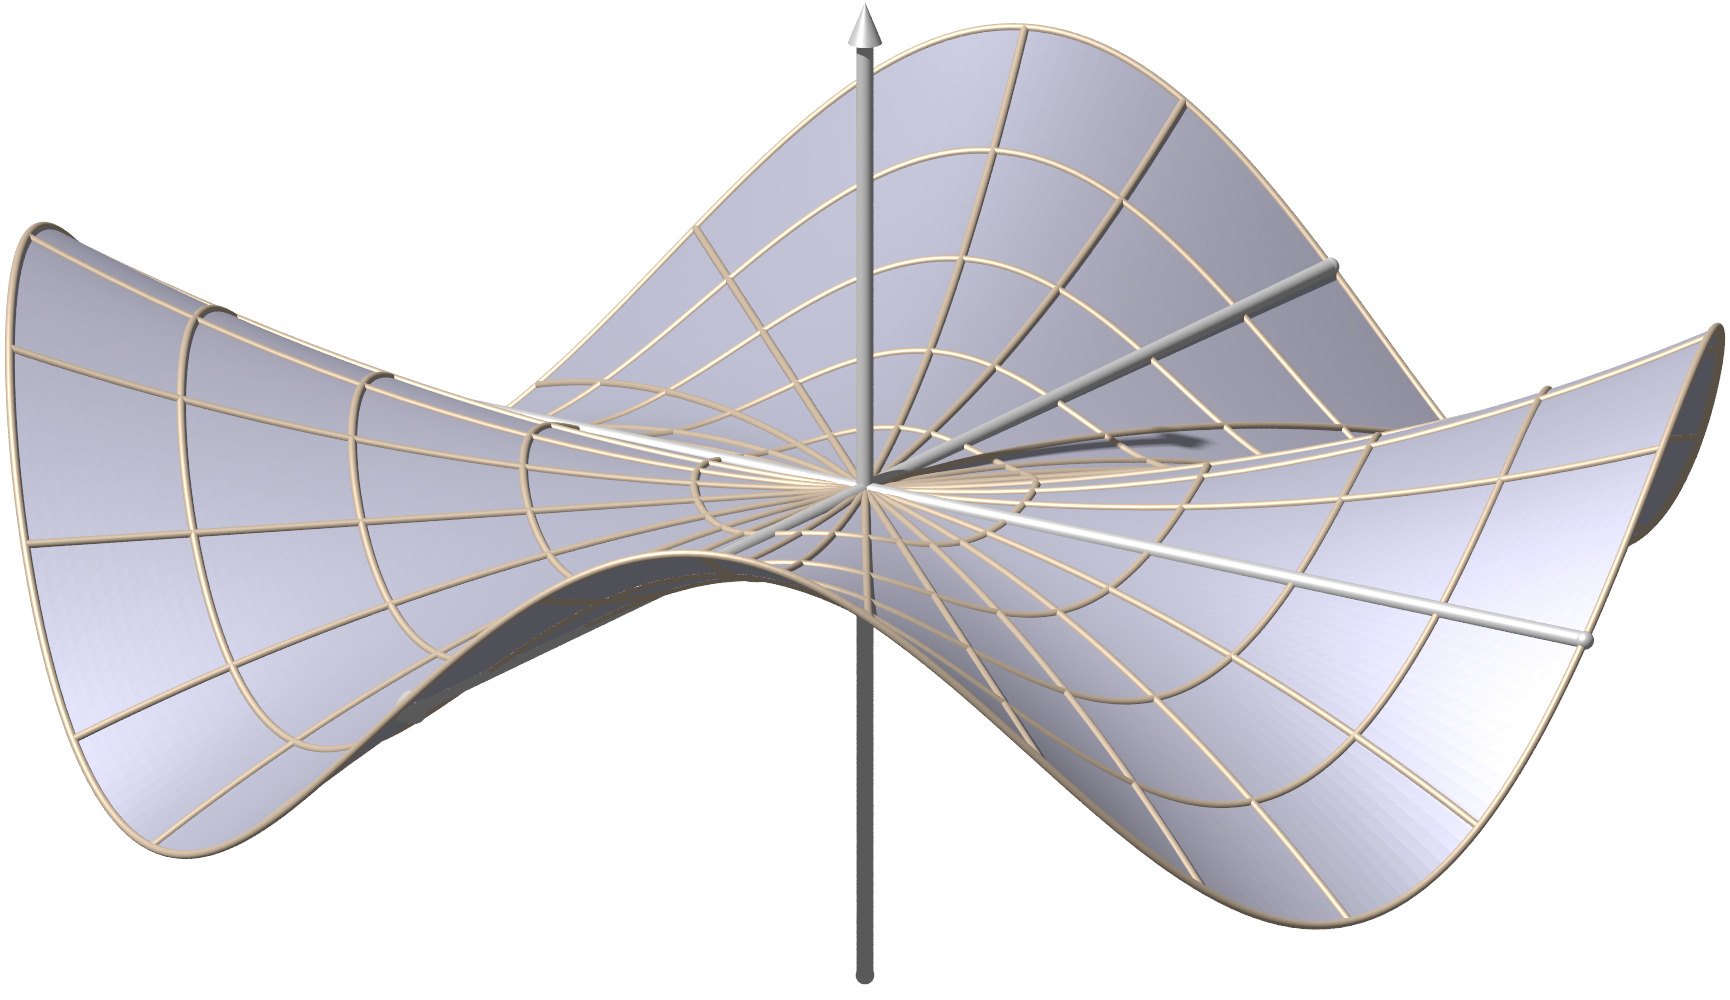
\includegraphics[width=\textwidth]{../slides/1/schwarz.jpg}
}
\only<2>{%
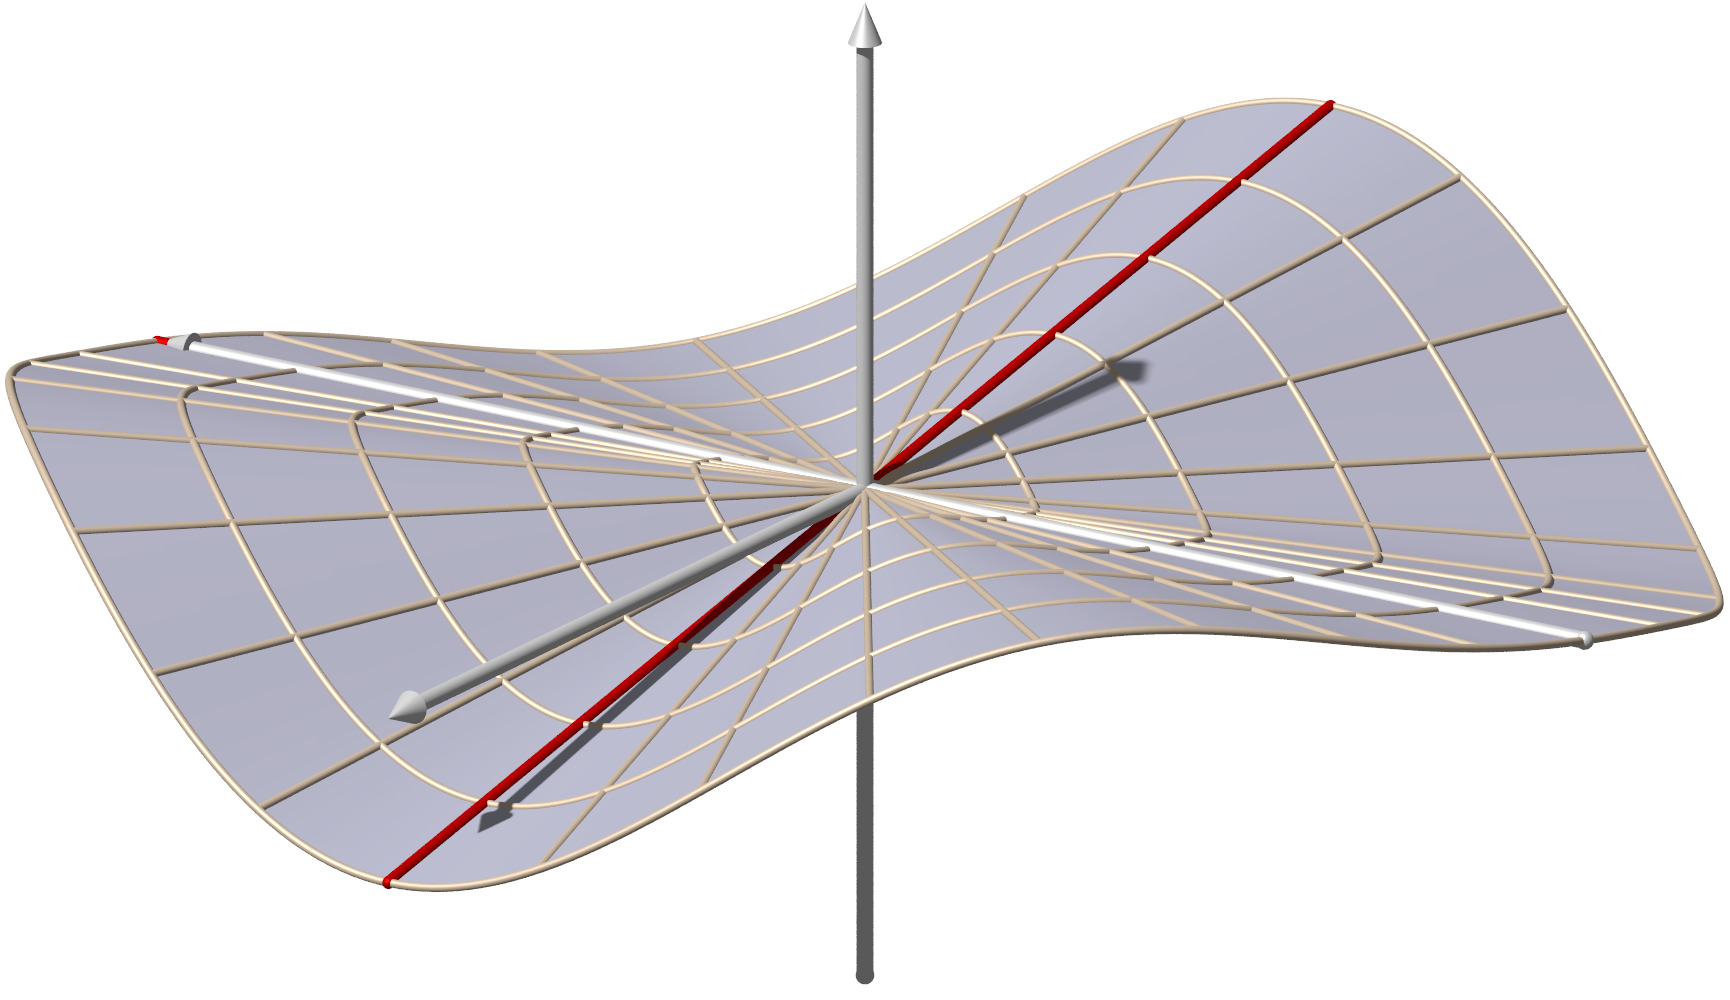
\includegraphics[width=\textwidth]{../slides/1/schwarzx.jpg}
}
\only<3>{%
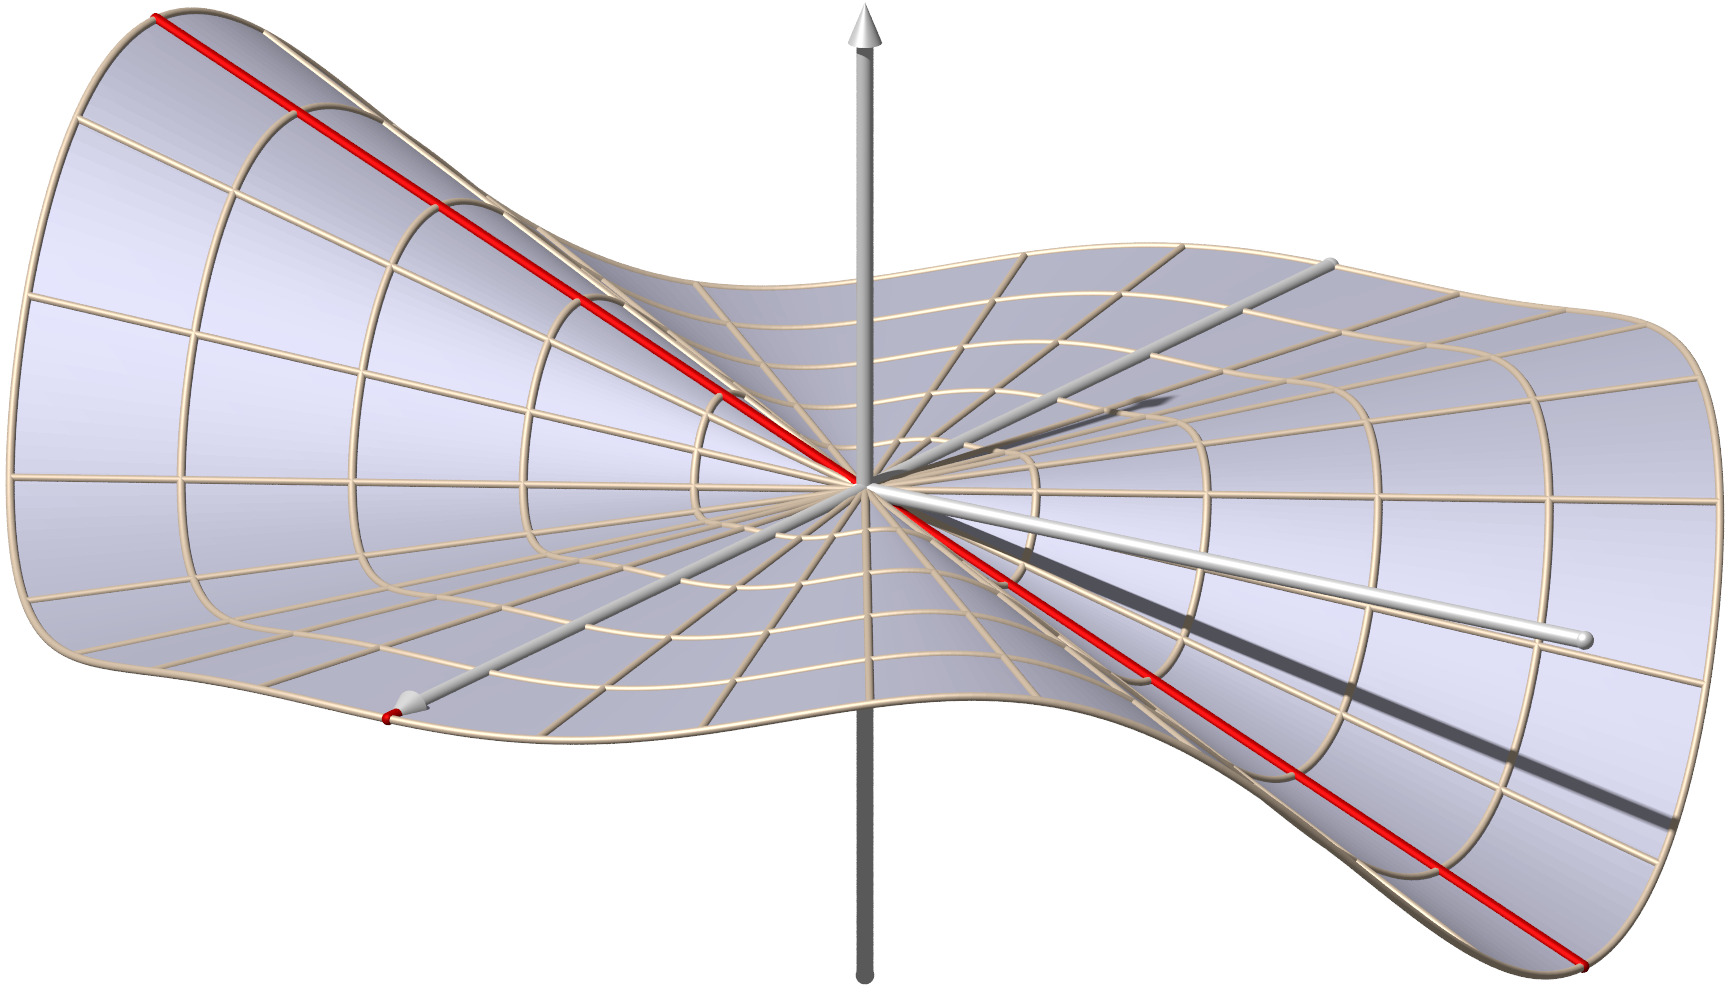
\includegraphics[width=\textwidth]{../slides/1/schwarzy.jpg}
}
\only<4>{%
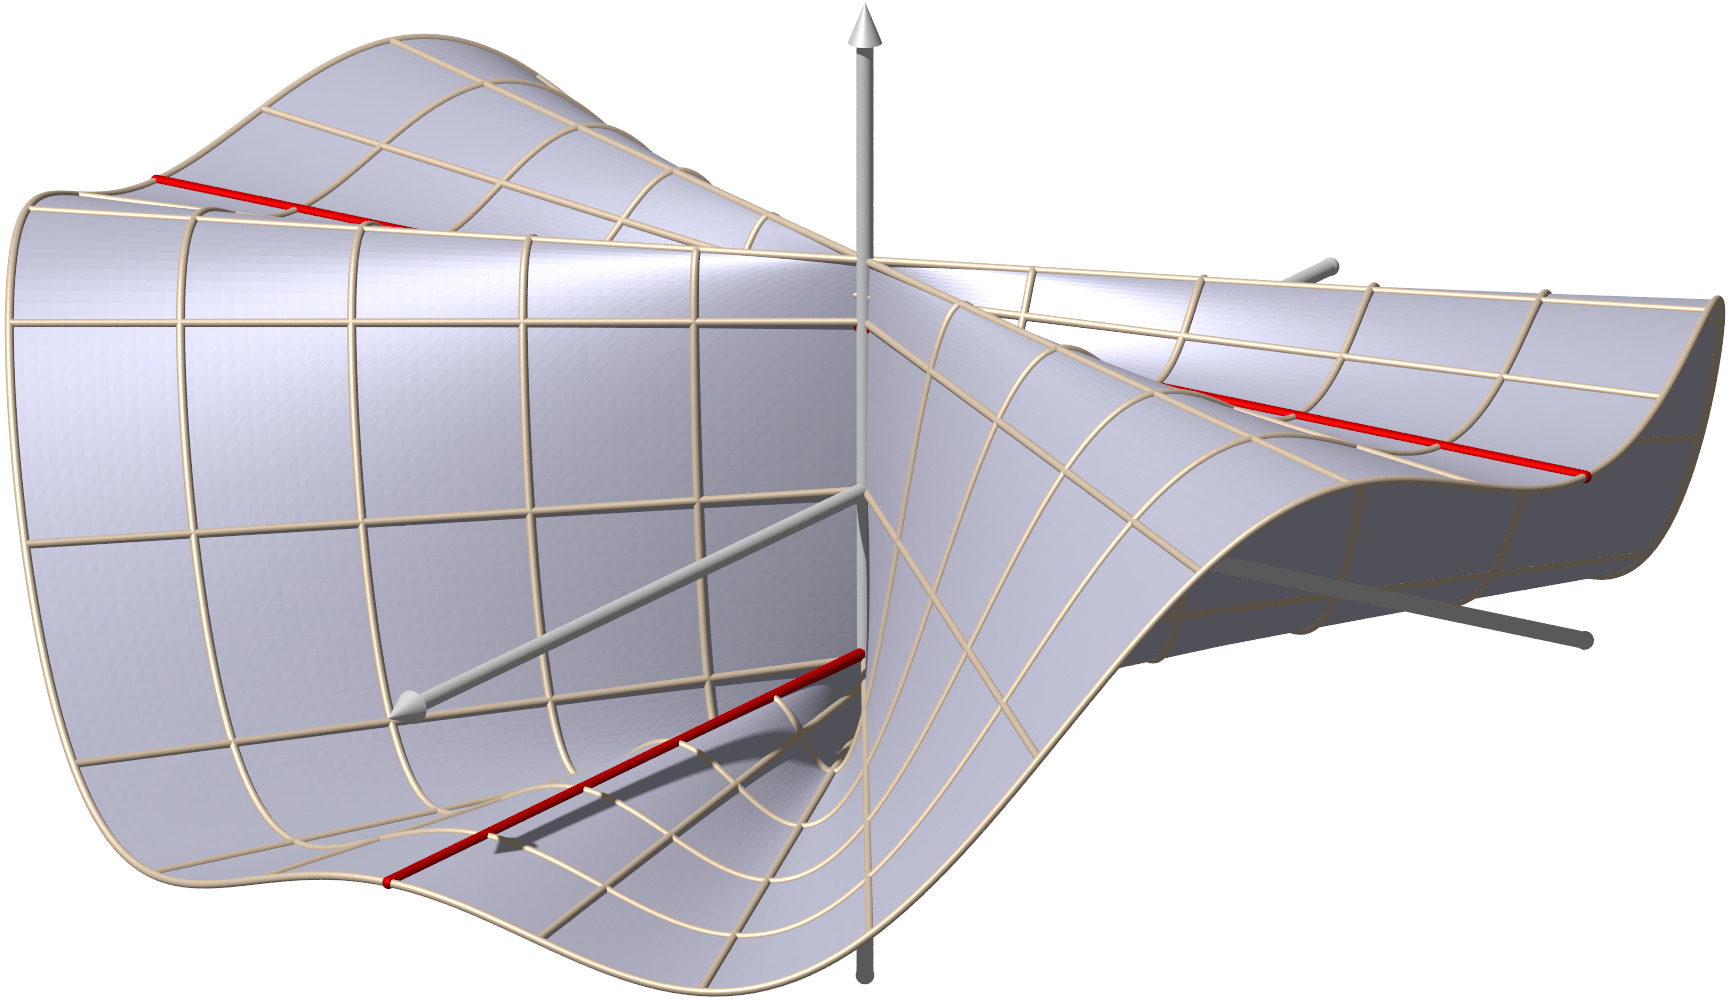
\includegraphics[width=\textwidth]{../slides/1/schwarzxy.jpg}
}
\end{frame}
\egroup
